
%%%%%%%%%%%%%%%%%%%%%%% file typeinst.tex %%%%%%%%%%%%%%%%%%%%%%%%%
%
% This is the LaTeX source for the instructions to authors using
% the LaTeX document class 'llncs.cls' for contributions to
% the Lecture Notes in Computer Sciences series.
% http://www.springer.com/lncs       Springer Heidelberg 2006/05/04
%
% It may be used as a template for your own input - copy it
% to a new file with a new name and use it as the basis
% for your article.
%
% NB: the document class 'llncs' has its own and detailed documentation, see
% ftp://ftp.springer.de/data/pubftp/pub/tex/latex/llncs/latex2e/llncsdoc.pdf
%
%%%%%%%%%%%%%%%%%%%%%%%%%%%%%%%%%%%%%%%%%%%%%%%%%%%%%%%%%%%%%%%%%%%


\documentclass[runningheads,a4paper]{llncs}

\usepackage{amssymb}
%\usepackage{amsthm}
\setcounter{tocdepth}{3}
\usepackage{graphicx}
\usepackage{booktabs}
\usepackage{todonotes}

\usepackage[font={small}]{caption, subfig}
%\usepackage{subcaption}
\usepackage{url}
\urldef{\mails}\path|{jlorince,pmtodd}@indiana.edu| 
\newcommand{\keywords}[1]{\par\addvspace\baselineskip
\noindent\keywordname\enspace\ignorespaces#1}

%\pdfpagesattr{/CropBox [94 112 523 778]}
  \def\baselinestretch{0.98}
  \addtolength{\textheight}{0.7in}
\begin{document}

\mainmatter  % start of an individual contribution

% first the title is needed
\title{Analysis of music tagging and listening patterns: Do tags really function as retrieval aids?}


% a short form should be given in case it is too long for the running head
\titlerunning{Do tags really function as retrieval aids?}

% the name(s) of the author(s) follow(s) next
%
% NB: Chinese authors should write their first names(s) in front of
% their surnames. This ensures that the names appear correctly in
% the running heads and the author index.
%
\author{Jared Lorince\inst{1}%
\and Kenneth Joseph\inst{2} \and Peter M. Todd\inst{1}}
%
\authorrunning{Lorince, Joseph, \& Todd}
% (feature abused for this document to repeat the title also on left hand pages)

% the affiliations are given next; don't give your e-mail address
% unless you accept that it will be published
\institute{Cognitive Science Program\\
%Department of Psychological \& Brain Sciences\\
Indiana University, Bloomington, Indiana, USA\\
\mails \\
\and 
Computation, Organization, and Society Program \\
%School of Computer Science\\
Carnegie Mellon University, Pittsburgh, PA, USA\\
\email{kjoseph@cs.cmu.edu}}

%
% NB: a more complex sample for affiliations and the mapping to the
% corresponding authors can be found in the file "llncs.dem"
% (search for the string "\mainmatter" where a contribution starts).
% "llncs.dem" accompanies the document class "llncs.cls".
%

\toctitle{Analysis of music tagging and listening patterns: Do tags really function as retrieval aids?}
\tocauthor{Lorince, Joseph, \& Todd}
\maketitle

\begin{abstract}
In collaborative tagging systems, it is generally assumed that users assign tags to facilitate retrieval of content at a later time. There is, however, little behavioral evidence that tags actually serve this purpose. Using a large-scale dataset from the social music website Last.fm, we explore here how patterns of music tagging and subsequent listening interact in an effort to determine if there exist measurable signals of tags functioning as retrieval aids. Specifically, we describe our methods for testing if the assignment of a tag tends to lead to an increase in listening behavior. Results suggest that there exists a small but reliable effect of tags increasing listening levels, and also reveal interesting differences in which kinds of tags are most associated with future listening.
\keywords{Collaborative tagging, Folksonomy, Music listening, Memory cues, Retrieval aids, Personal information management}
\end{abstract}
\setcounter{footnote}{0}


\section{Introduction}
\label{sec_intro}

In social tagging systems, users assign freeform textual labels to digital content (music, photos, web bookmarks, etc.). There are a variety of reasons for which users tag content, but it is overwhelmingly assumed that tagging for one's own future retrieval -- assigning a tag to an item to facilitate re-finding it at a later time -- is users' principal motivator. But is this a valid assumption?
%These individual tagging decisions can be aggregated into a folksonomy \cite{VanderWal2007}, a ``bottom-up'' classificatory structure developed with little or no top-down guidance or constraints.

Collaborative tagging systems are often designed, at least in part, as resource management platforms that expressly facilitate the use of tags as retrieval aids.  However, the freeform, and often social, nature of tagging opens up many other possible reasons for which a user might tag a resource. While there is a significant amount of non-controversial evidence for such alternative tagging motivations, (sharing resources with other users, social opinion expression, etc.), the problem with the retrieval aid assumption runs deeper than there simply existing possible alternatives. There is, in fact, almost no behavioral evidence that tags are ever actually used as retrieval aids. While there is much data available on user tagging habits (i.e. which terms are applied to which resources, and when), to our knowledge there is no published research providing behavioral evidence of whether or not tags, once applied to items, actually facilitate subsequent retrieval. This is an issue largely driven by a lack of data: while a web service can in principle track a users' interaction with tags (for instance, if users use tags as search terms to find tagged content), there are no available datasets containing such information, nor can it be crawled externally by researchers.

Despite these issues, this empirical question is not intractable. While detailed information on how existing tags are utilized remains beyond our reach, an alternative approach is to examine how patterns of user interaction with tagged versus untagged content vary. If tags do serve as retrieval aids, we should expect users to be more likely to interact with a resource (e.g. visit bookmarked pages, listen to songs, view photos, etc.) once they have assigned a tag to it.

Here we test this hypothesis using a large-scale dataset consisting of complete listening and tagging histories from more than 100,000 users from the social music website Last.fm. From this dataset, we extract user-artist listening time-series, each of which represents the frequency of listening over 90 months to a particular artist by a particular user, and compare time-series in which the user has tagged the artist to those that are untagged. Specifically, we address the following two questions:
\begin{itemize}
	\item {\bf RQ1}: Does tagging an artist increases the probability of listening to that artist in the future, as shown by comparison of tagged versus untagged time-series?
	\item {\bf RQ2}: Are certain tags particularly associated with increases in future listening, and if so, can we identify attributes of such ``retrieval-targeted'' tags as opposed to others?
\end{itemize}

%We describe the various analytic methods we bring to bear on these questions in Section~\ref{sec_analyses}, but first present related work (Section~\ref{sec_related}) and details of our dataset (Section~\ref{sec_dataset}). We close in Section~\ref{sec_conclusion} with synthesis and interpretation of our results, as well as a plan for future work.
\section{Background}
\label{sec_related}

\subsection{The formal study of folksonomies}
Collaborative tagging has been considered one of the core technologies of ``Web 2.0'', and has been implemented for resources as diverse as web bookmarks (Delicious), photos (Flickr), books (LibraryThing), academic papers (Mendeley), and more. Vander Wal \cite{VanderWal2007} coined the term ``folksonomy'' to describe the emergent semantic structure defined by the aggregation of many individual users' tagging decisions in such a system. These folksonomies have since become the target of much academic research. One of the earliest analyses of a collaborative tagging system is Golder and Huberman's \cite{Golder2006} work on the evolution of tagging on Delicious.com.  Around the same time, Hotho and colleagues \cite{Hotho2006a} presented a formal definition of a folksonomy: $\mathbb{F} := (U,T,R,Y)$ \footnote{This is a slight simplification. For details, see \cite{Hotho2006a}}. The variables $U$, $T$, and $R$ represent, respectively, the sets of users, tags, and resources in a tagging system, while $Y$ is a ternary relation between them ($Y \subseteq U \times T \times R$). The ``personomy'' of a particular user (i.e. the set of annotations generated by an individual),  $\mathbb{P} := (T_{u},R_{u},Y_{u})$, can be similarly defined.

Since 2006, an extensive literature on \emph{how} people tag has also developed, covering topics like tagging expertise \cite{Yeung2011},	mathematical \cite{Cattuto2007a} and multi-agent \cite{Lorince2013} models of tagging choices, consensus in collaborative tagging \cite{Halpin2007,Robu2009}, and much more. Our understanding of the dynamics of tagging behavior has greatly expanded, but understanding exactly \emph{why} people tag, on the other hand, has proven more elusive.

\subsection{Why do people tag?}
It is typically assumed that tags serve as retrieval aids, allowing users to re-find content to which they have applied a given tag (e.g. a user could click on or search for the tag ``rock'' to retrieve the songs she has previously tagged with that term). This assumption is baked into Vander Wal's original defintion of a folksonomy, which he contends ``is the result of personal free tagging of information and objects (anything with a URL) \emph{for one's own retrieval}'' \cite[emphasis added]{VanderWal2007}. This perspective is echoed in many studies of tagging patterns \cite{Glushko2008,Halpin2007,Golder2006}.

But while retrieval is the most commonly assumed motivation for tagging, other reasons certainly exist, and various researchers have developed taxonomies of tagging motivation. Among proposed motivational factors in tagging are personal information management (including but not limited to tagging for future retrieval), resource sharing, opinion expression, performance, and activism \cite{Heckner2009,Zollers2007,Ames2007}, among others. See \cite{Gupta2010} for a review.

While the development of motivational theories in tagging is useful, there is almost no work actually grounding them in behavioral observations. The vast majority of existing work either makes inferences about motivation based on design features of a website (e.g. social motivations in tagging require that one's tags be visible to other users, \cite{Marlow2006}), employs semantic analysis and categorization of tags (e.g. the tags ``to read'', ``classical'', and ``love'' can all be inferred to have different uses, \cite{Zollers2007,Sen2006}), or directly asks users why they tag using survey methods \cite{Ames2007,Nov2008}. The results of such approaches are useful contributions to the field, but few have resulted in testable behavioral hypotheses that can confirm or refute their validity.

One notable exception is work by K\"{o}rner and colleagues \cite{Korner2010,Korner2010a,Zubiaga2011}. They argue that taggers can be classified on a motivational spectrum from categorizers (who use a constrained vocabulary suitable to future browsing of their own tagged resources) to describers (who use a large, varied vocabulary to facilitate future keyword-based search using their own tags), and have developed and tested quantifiable signals of these different motivations. The main deficiency of this approach, however, is that their hypotheses are based fully on attributes of user tag vocabularies; they present no way to test whether or not describers actually use tags, once applied, for keyword-based search and that categorizers use them for browsing.

Again, the problem of lack of verification arises because data on how users actually \emph{use} existing tags is simply not available to researchers through any tagging system APIs (or through other methods) that we are aware of. Thus the existing work on tagging motivation is limited to inferring \emph{why} people tag from \emph{how} they tag, rather than from how they \emph{use} their tags. In presenting our novel methods, we are aware that they still represent an inferential approach. Our approach is distinct from those described here, however, in that we test a concrete hypothesis about how tagging should affect a behavior on which we \emph{do} have data (interaction with tagged content, in our case music listening).
%\subsection{Insights from cognitive science}
\section{Dataset}
\label{sec_dataset}
Last.fm incorporates two specific features of interest to us here. First, it implements a collaborative tagging system (a ``broad'' folksonomy, following Vander Wal's \cite{VanderWal2005} terminology, meaning that multiple users tag the same, publicly available content) in which users can label artist, albums, and songs. Second, the service tracks users' listening habits both on the website itself and on media players (e.g. iTunes) via a software plugin. This tracking process is known as ``scrobbling'', and each timestamped instance of a user listening to a particular song is termed a ``scrobble''.

Here we utilize an expanded version of a dataset described in earlier work \cite{Lorince2013,Lorince2014} that includes the full tagging histories of approximately 1.9 million Last.fm users, and full listening histories from a subset of those users (approximately 100,000) for a 90-month time window (July 2005 - December 2012, inclusive). Data were collected via a combination of the Last.fm API and direct scraping of publicly available user profile pages. For further details of the crawling process, see \cite{Lorince2013,Lorince2014}.

For our current purposes, we consider only those users for which we have both tagging and listening histories. For each user, we extract one time series for each unique artist listened to by that user. Each user-artist listening time series consists of a given users's monthly listening frequency to a particular artist for each month in our data collection period, represented as a 90-element vector. 

The over 2 billion individual scrobbles in our dataset define a total of XXX such time series. In XXX of these cases, the user has assigned at least one tag to the artist within the collection period (we refer to these as tagged time series), while in the remaining cases (XXX) the user has never tagged the artist. We summarize these high level dataset statistics in Table~\ref{tab:data_summary}.

\begin{table}[h]
\begin{center}
\begin{tabular}{l|r}
\toprule
Total users & 104,829 \\
Total scrobbles & 2,089,473,214 \\
Unique artists listened & X,XXX,XXX \\
Unique artists tagged & X,XXX,XXX \\
\midrule
Total user-artist listening time series & XX,XXX,XXX \\
Total tagged time series & X,XXX,XXX \\
Total untagged time series & 88,944,512 \\
\bottomrule
\end{tabular}
\end{center}
\caption{Dataset summary}
\label{tab:data_summary}
\end{table}
\section{Analyses \& Results}
\label{sec_analyses}

\subsection{RQ1: Comparison of tagged and untagged time-series}
Our principal research question is whether listening patterns for tagged content are consistent with the expectation that tags serve as memory cues. If this were to be the case, we would expect to see an increase in a user's listening rate to musical artists after the user has tagged them, under the assumption that a tag facilitates retrieval and increases the chances of a user listening to a tagged artist. 

Unfortunately, several factors combine to make such an analysis difficult.  First and foremost, the desired counterfactual of the untagged ``version'' of a particular tagged series, which would allow a direct testing of how tagging changes listening behavior, does not, of course, exist. We thus must utilize untagged time-series in a way that allows them to approximate what a true counterfactual might look like.  In searching for such samples, a second difficulty that arises is that listening rates for tagged time-series are much greater than for untagged time-series (the average number of total listens across time-series is 16.9 when untagged and 98.9 when tagged). While suggestive of the importance of tagging, this unbalance also suggests that controls must be instilled in both sample selection and statistical analysis to account for previous listening behavior prior to tagging. Finally, the actual point in time at which tags are expected to increase listening behavior for any given user is unknown. Thus, we must formulate our analysis to account for this uncertainty.  
%to understand how it changes behavior
%as it is theoretically possible that tagging may affect listening behavior as much three months after the tag has been placed as it does in the immediately following month.

%meticulously
To alleviate issues with the non-existence of a true counterfactual, we subselect from both the tagged and untagged series using the following formal procedure. We first temporally align the tagged and untagged time-series by selecting only those tagged time-series where the tag was applied in the month of peak listening and aligning them at that peak point, and then collecting a sample of untagged time-series also aligned at the peak of listening.  Where the peak was reached in multiple months, we chose one of these at random.
%Both tagged time-series are aligned so that they are centered on the month in which they were tagged.  If multiple tags were present, we selected the tag within the month which had the most corresponding scrobbles. While there is no analogue to this point in the untagged data, we can partially resolve the issue by noting that tagging is disproportionately likely (approximately 30\%, compared to 1.1\% if the tagging month were random) to occur in a user's \emph{peak}\footnote{The month in which they listen the most times overall} listening month for a given artist. This provides a basis for aligning the tagged and untagged time-series,

%while still admitting that there is likely a reasonable span in which tagging and past listening behavior have an effect on future actions
After aligning all tagged and untagged samples in this fashion, we further limited our analysis to a 13 month period extending from 6 months prior to the peak month to 6 months after the peak. This allows us to consider a variety of ways in which listening prior to the tag may affect future behavior. Finally, we further constrain our sampling to time-series with:
\begin{itemize}
\vspace{-.5em}
\item more than 25 total listens; 
\item a peak in listening at least 6 months from the edges of our data collection period (i.e. ensuring that the period from 6 months before to 6 months after the peak does not extend beyond the limits of our data range); and
\item at least one listen 6 months prior to and after the peak (i.e. if the peak occurs in July, there should be at least one listen between January and June, and one between August and the following January).
\vspace{-.5em}
\end{itemize}

Constraining our time-series in this manner, we are left with a total of 206,140 tagged time-series.  We then randomly sampled from the 4.1M untagged time-series an equal number meeting the same three criteria.  All results below have been verified with multiple random samplings of the untagged data.

In Figure~\ref{fig:taggedVsUntagged} we plot mean playcounts, with 95\% normal confidence intervals, for each month across all tagged and untagged time-series in the subsampled data. All values are normalized by the peak, and thus values at the peak month for both the tagged and untagged lines are unity. By visually comparing the line heights before and after the peak, Figure~\ref{fig:taggedVsUntagged} shows that the mean normalized listening rate increases in the months after the peak for both tagged and untagged time-series. However, we also see a small but reliable effect wherein tagged time-series show proportionally higher mean normalized listening rates after the peak month (in which the the tag was applied) as compared to untagged time-series. This is suggestive of an increase in listening as a result of tagging.\footnote{We also observe, however, that an small but reliable lower rate of listening to tagged artist prior to peak listening. This may indicate that songs that ``catch on'' for a user more quickly (rise faster in listening from before the peak to the peak) are more likely to be tagged, a possibility to be explored further in future work.}

While Figure~\ref{fig:taggedVsUntagged} thus gives evidence that supports our hypothesis, there are two important caveats. First, as the distribution of the number of listens in any given month across all time series is heavily skewed, the mean is not fully representative of the data. Though qualitative plots of transformed variables proved to be similar, our further statistical analysis uses a log transformed version of the listening counts to account for these deviations. Second, it seems intuitively important to control for the effect of pre-peak listening behavior on post-peak listening.

 To more robustly test our hypothesis, we therefore use a regression model that incorporates previous listening behavior on post-peak behavior. Due to a lack of knowledge about the relationship between these variables and the volume of data we have, it was both unreasonable and unnecessary to assume a linear relationship between the dependent and independent variables. Because of this, we opted for a Generalized Additive Model (GAM, \cite{hastie1990generalized}) using the R package mgcv \cite{wood2001mgcv}. Our dependent variable in the regression is the logarithm of the sum of all listens in the six months after a tag has been applied, to capture the possible effect of tagging over a wide temporal window. Note, however, that qualitative results hold when testing listening for each individual month as well.
% Also of note is our choice of using the log of the dependent variable rather than a count-based regression model (e.g. a Negative Binomial regression). The model used here appeared to fit the data better based on a variety of statistical and visual goodness-of-fit tests.
Our independent variables are a binary indicator of whether or not the time-series has been tagged, as well seven continuous-valued predictors, one each for the logarithm of the sum of listens in the peak month and the six previous months.   

  \begin{figure}[t]
    \subfloat[\label{fig:taggedVsUntagged}]{%
      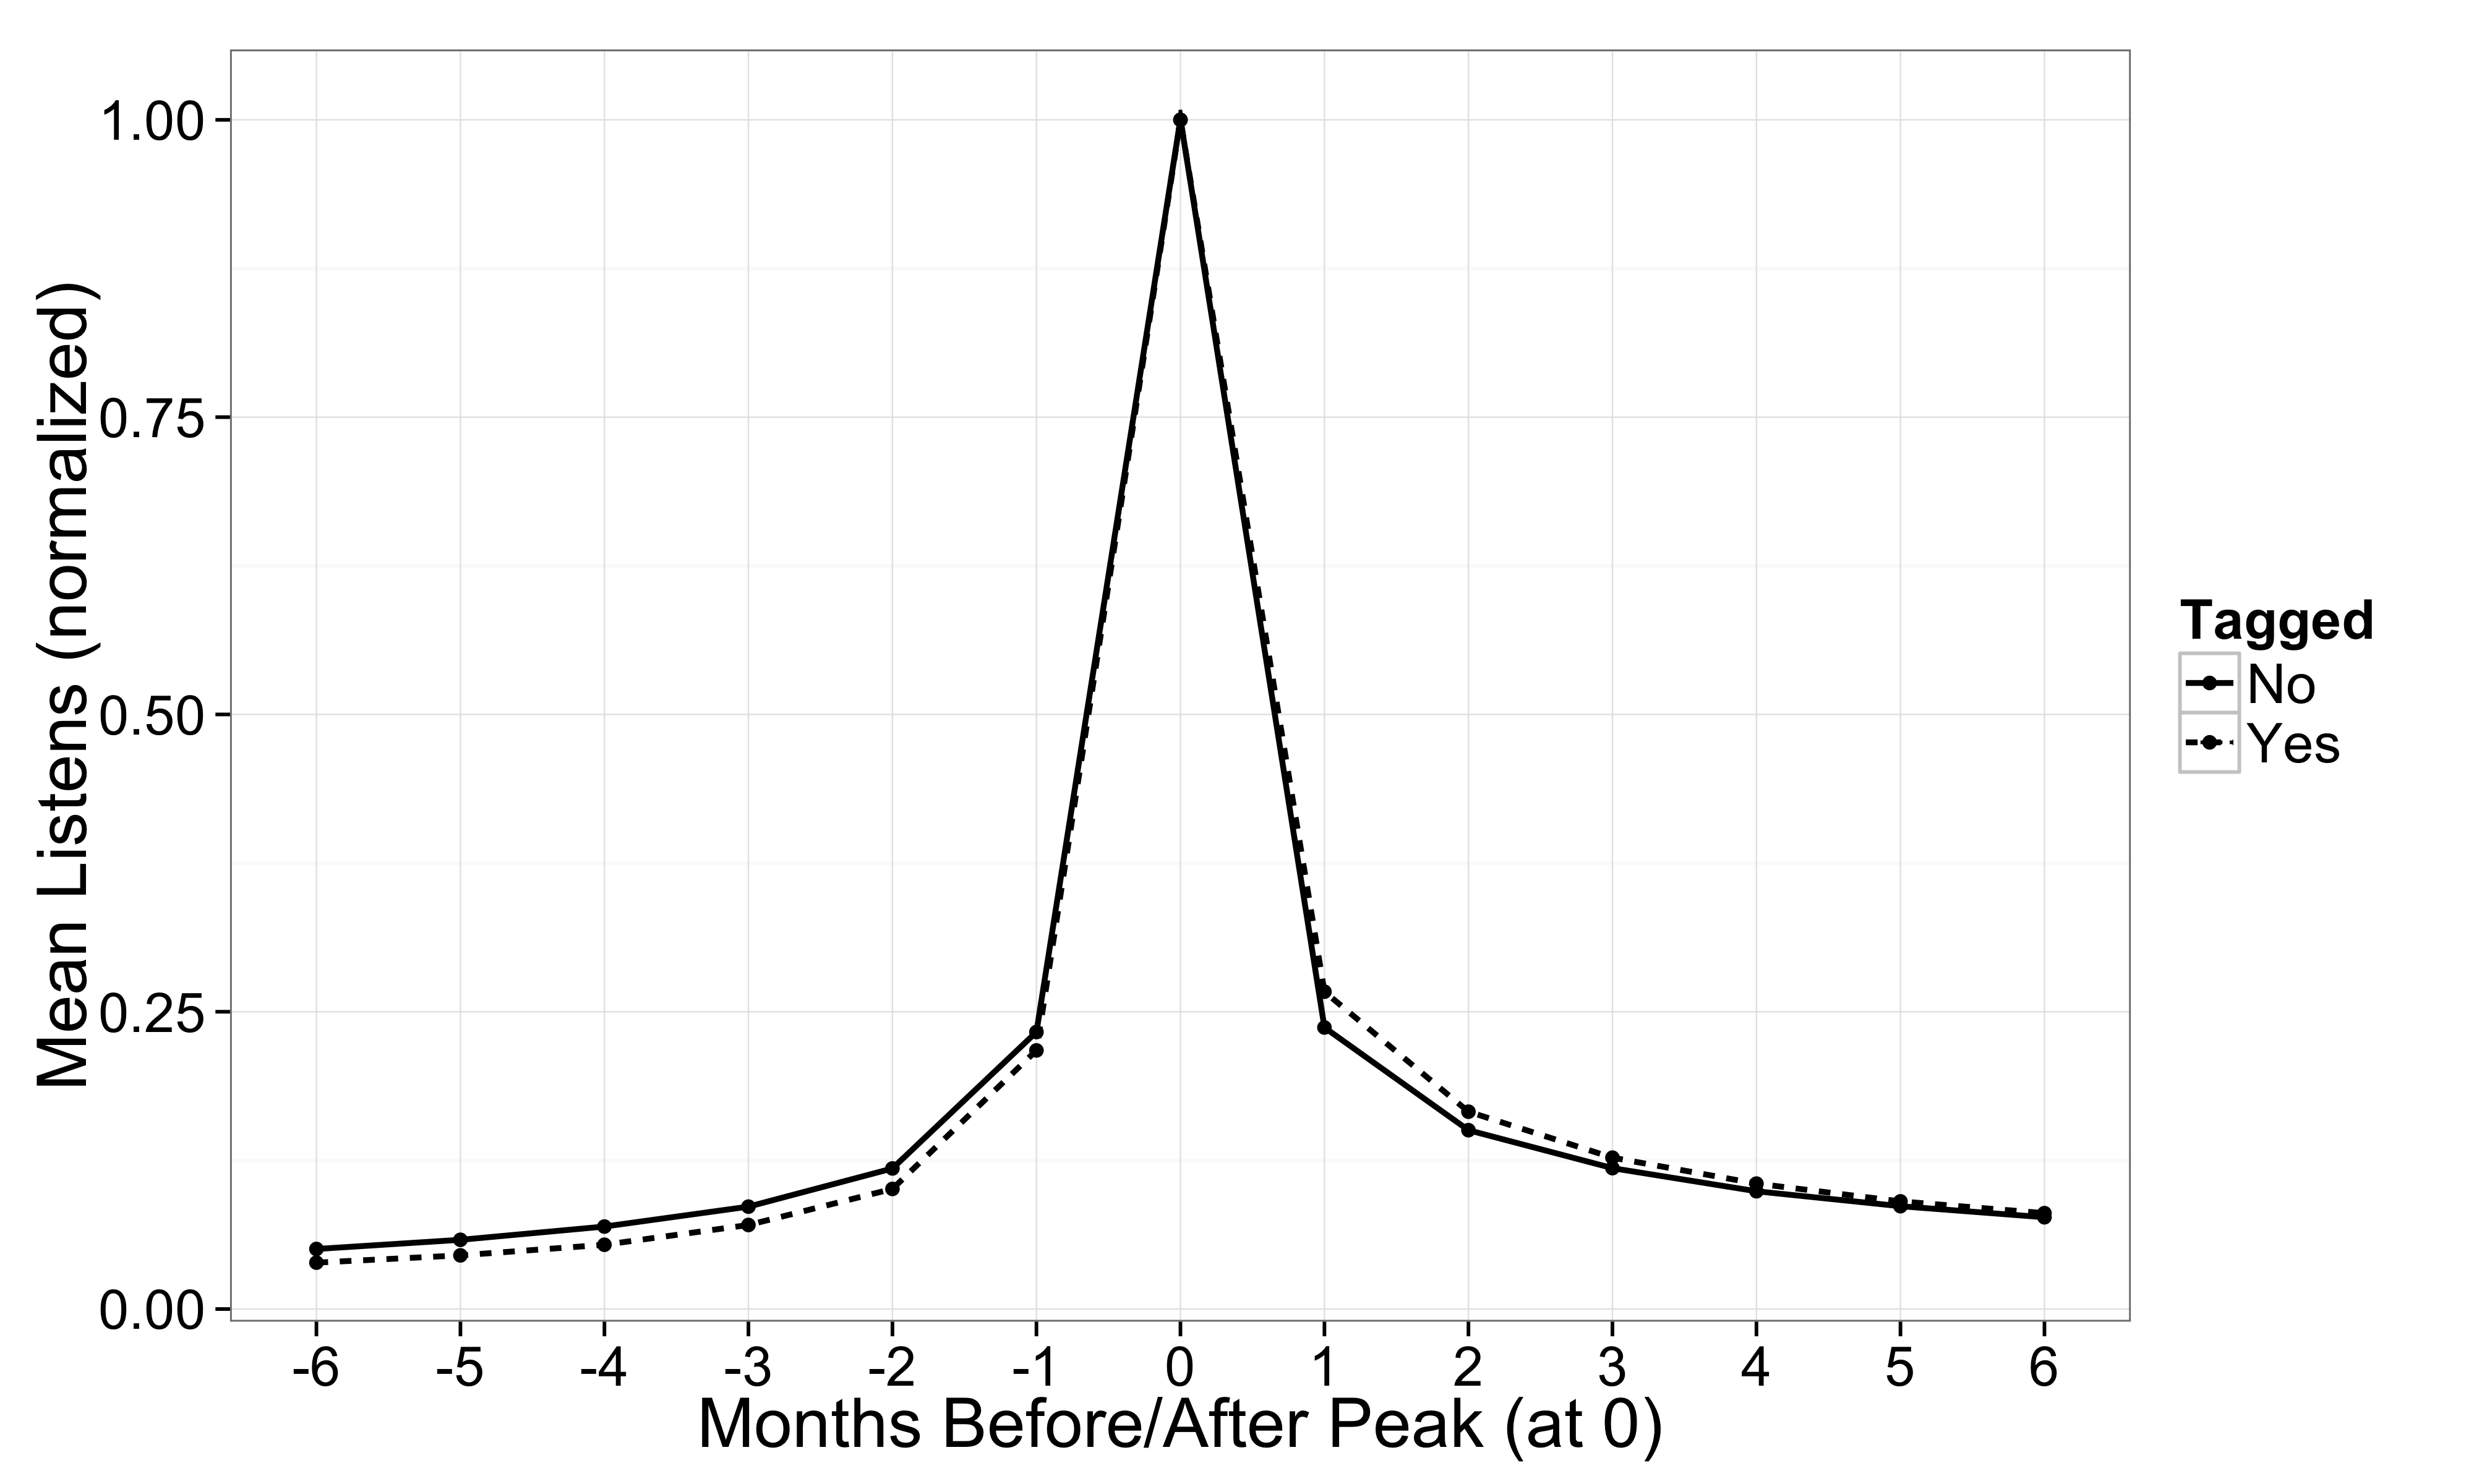
\includegraphics[width=0.45\textwidth]{taggedVUntaggedSimple.png}
    }
    \hfill
    \subfloat[\label{fig:regression}]{%
      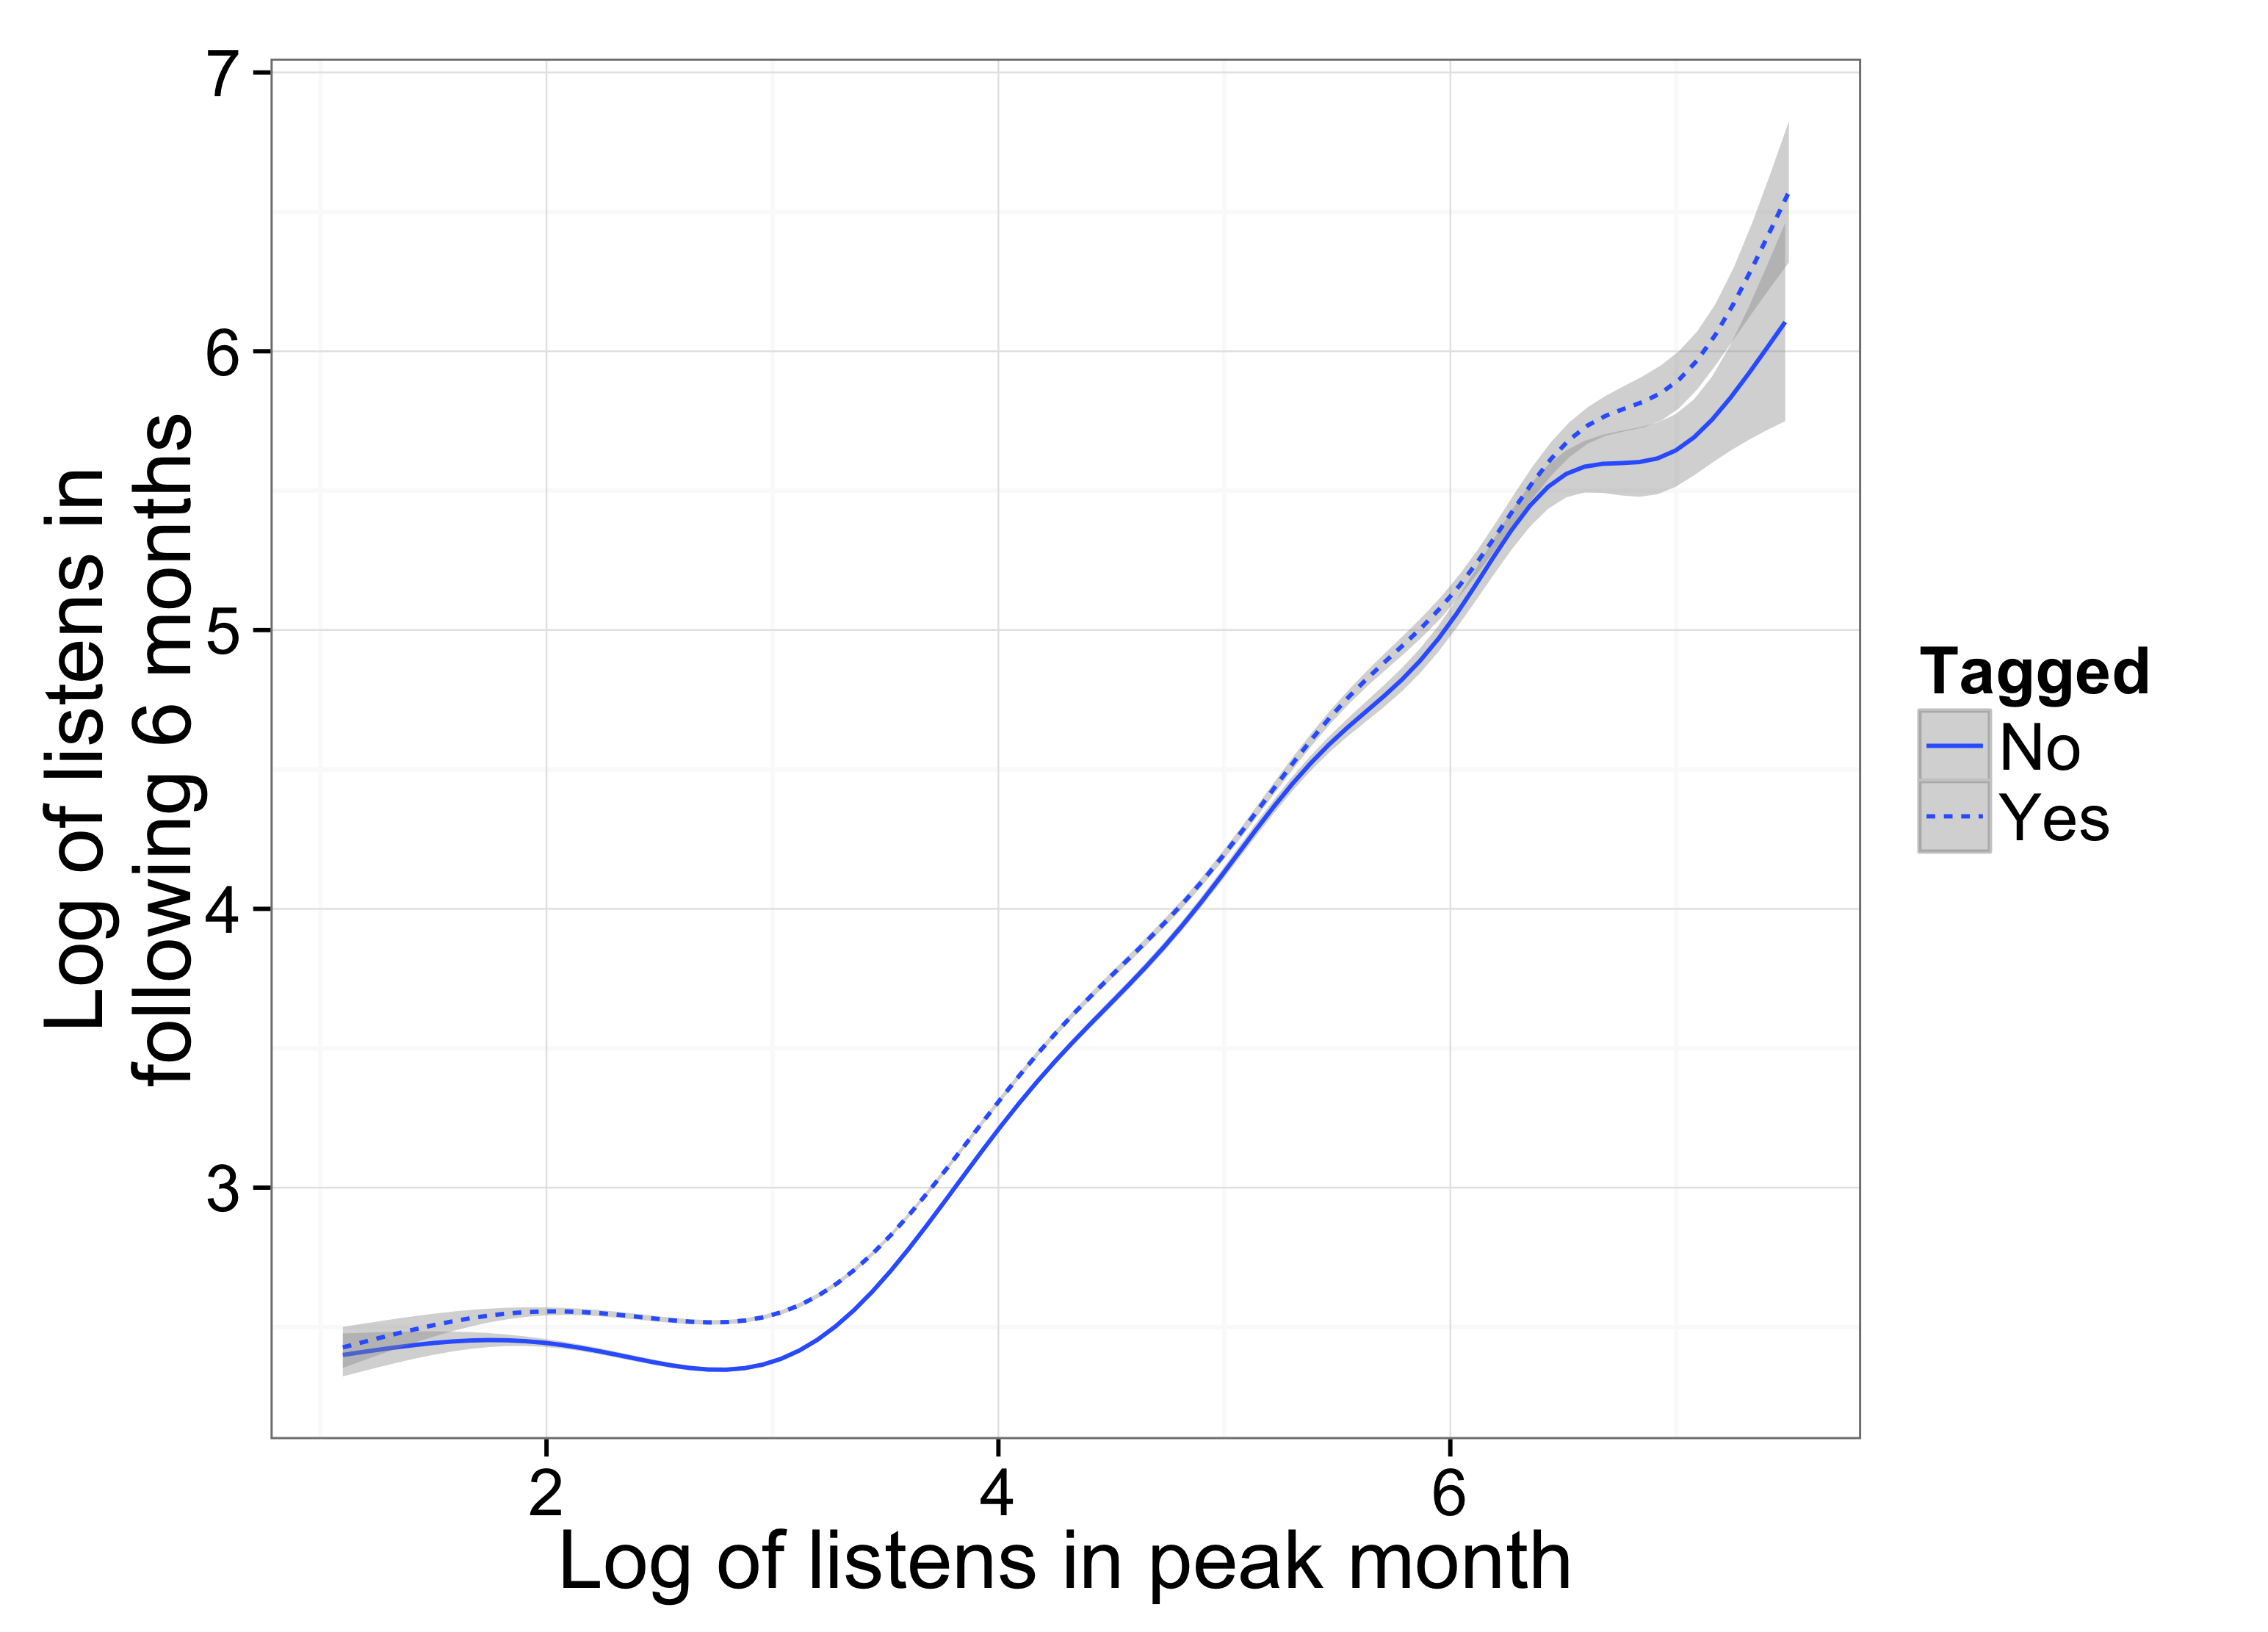
\includegraphics[width=0.45\textwidth]{taggedVUntaggedRegression.png}
    }
    \caption{Comparison of tagged and untagged listening time-series. Mean normalized playcount by month (a), and Regression results, with 95\% confidence interval (b).}
    \label{fig:regressionFigs}
    \vspace{-2em}
  \end{figure}

The regression model, which explained approximately 30\% of the variance in the data (adjusted $R^{2}$), indicated that the tagged/untagged indicator, as well as listening rate parameters (smoothed using thin-plate regression splines) for all seven previous months had a significant effect on post-peak listening behavior ($P \ll 0.0001$). As we cannot show the form of this effect for all model variables at once, Figure~\ref{fig:regression} instead displays a similar model which considers only the effect of listening in the peak month on post-peak listening. As this plot suggests and the full model confirms, we can conclude that, controlling for all previous listening behavior, a tag increases the logarithm of post-peak listens by .147 (95\% CI = [.144,.150]). This indicates that the effect of a tag is associated with around 1.15 more listens over six months, on average, than if it were not to have been applied.   

\subsection{RQ2: Tag analysis}
To examine if and how different tags are associated with increased future listening, we ran a regression analysis similar to that described above, but with two important changes. First, instead of a single tagged/untagged indicator, we included binary (present / not present) regressors for the 1,231 unique tags that had at least five occurrences in our subsample\footnote{We choose a threshold of five to ensure that data was not too sparse for the regression model but in a way that still was inclusive of infrequently occurring tags.  Again, however, we note that qualitative results hold when using both more and less restrictive thresholds.} Second, due to the data-hungry nature of the GAM and the large number of additional variables introduced by utilizing all tags as unique predictors, we chose to only use listening in the peak month (for each tag) as the independent variables. This decision limited the computational difficulties associated with estimating a model of this size and did not appear to affect model fit substantially according to tests we ran on subsamples of the data. The same data were used as in the previous analysis (untagged time series, of course, had values of zero for all possible tags).
%Four important changes were made. First, we considered only tagged time-series.  Second, instead of a single tagged/untagged indicator, we included binary (present / not present) regressors for all unique tags that had at least five occurrences in our subsample\footnote{We choose a threshold of five to ensure that data was not too sparse for the regression model but in a way that still was inclusive of infrequently occurring tags.  Again, however, we note that qualitative results hold when using both more and less restrictive thresholds.}. Third, due to the data-hungry nature of the GAM and the large number of additional variables introduced by utilizing all tags as unique predictors, we chose to only use listening in the peak month (for each tag) as the independent variables. This decision limited the computational difficulties associated with estimating a model of this size and did not appear to affect model fit substantially according to tests we ran on subsamples of the data. Finally, we eliminated the constraint that a tag must occur in the peak month of a time-series, as there is no meaningful comparison to be made with untagged data in this analysis. This allowed us to include additional tagged time-series. The dependent variable remained the log number of listens in the 6 months following tagging. If users had multiple tags for a particular artist, we again selected one tag randomly rather than include the same user artist combination twice in our analysis.

After running the model, which explains approximately 29\% of the variance in the data (adjusted $R^{2}$), 136 unique tags were statistically significant predictors at $\alpha =.001$, which we selected in order to account for the large number of comparisons against the null hypothesis being made in the regression model. While we only have sufficient evidence to make claims about these 136 tags,\footnote{Note, however, that the qualitative trends observable in the plots to follow hold regardless of the $\alpha$ threshold used.} qualitative examination of which tags are relatively strong predictors in the model proved informative.

Unsurprisinlgly, most tags tend to have a positive (albeit small) impact on future listening, as evidenced by positive regression coefficients and consistent with the small positive effect of tagging observed overall in the previous analysis. The most telling observation is that commonly-used genre tags (e.g. ``pop'', ``jazz'', and ``hip-hop'') -- which are the most common tags overall in our full dataset -- tend to be weak, positive predictors of future listening. In contrast, relatively strong predictors (both positive and negative) appear to be comparatively obscure, possibly idiosyncratic tags (e.g. ``cd collection'', ``mymusic'', ``purchased 09'').\footnote{For a full listing of the regression coefficients across all tags in the model, see \url{https://dl.dropboxusercontent.com/u/625604/papers/lorince.joseph.todd.2015.sbp.supplemental/regression_coefficients.txt}} To examine this trend quantitatively, we plot in Figure~\ref{fig:coefVsPopularity} the global tag popularity (i.e. the total number of uses of a tag in our full dataset of approximately 50 million annotations) as a function of the tag's impact on listening as indicated by its coefficient in the regression model. Similarly, we plot in Figure~\ref{fig:coefVsPopularityPeople} the unique number of users utilizing the tag, again as a function of the regression coefficients of statistically significant predictors. The value of $e^c$, where $c$ is the value of a regression coefficient, represents the number of listens we expect user's post-listening behavior to increase or decrease by if the given tag were to be applied (thus the strongest predictors lead to an increase of approximately 4.5 listens on average). Finally, in each plot, the red bands marked the upper and lower limits of a bootstrapped 95\% confidence interval on the popularity of the 1,095 remaining tags that were \emph{not} significant in the regression model. 
%, for all tags that had a statistically significant coefficient.
  \begin{figure}[t]
    \subfloat[\label{fig:coefVsPopularity}]{%
      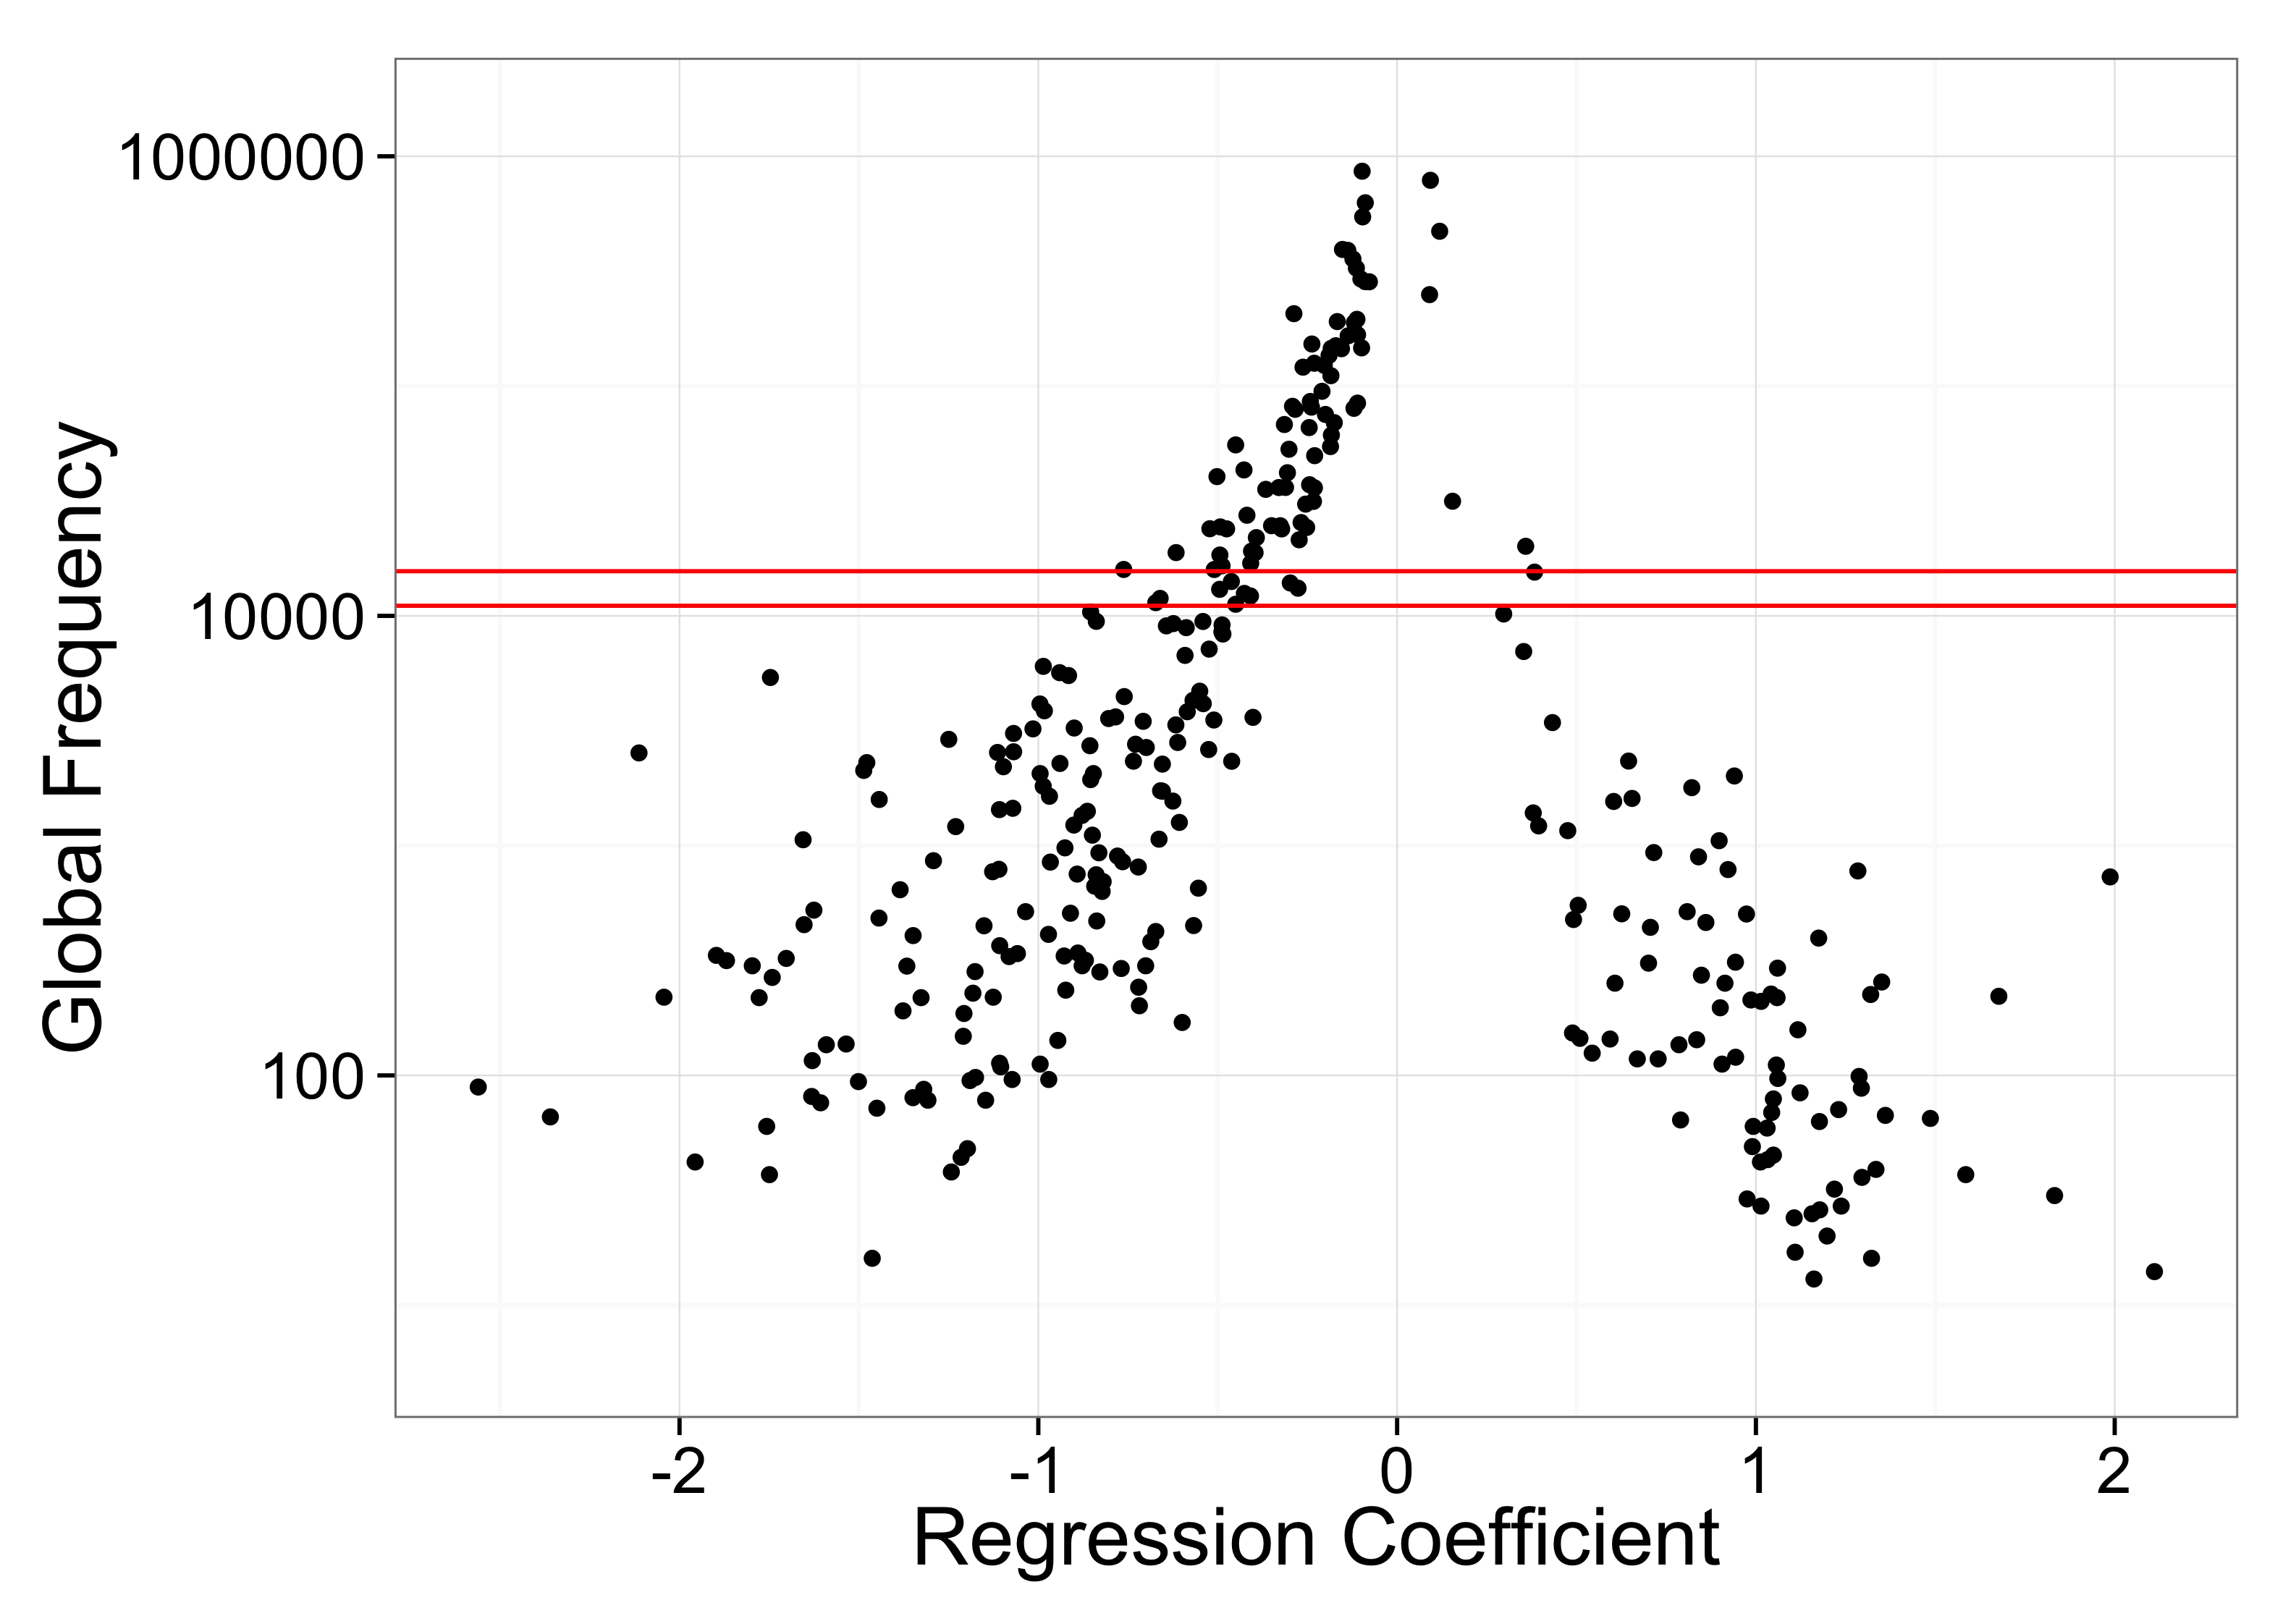
\includegraphics[width=0.45\textwidth]{tagRegressionWithMoreData.png}
    }
    \hfill
    \subfloat[\label{fig:coefVsPopularityPeople}]{%
      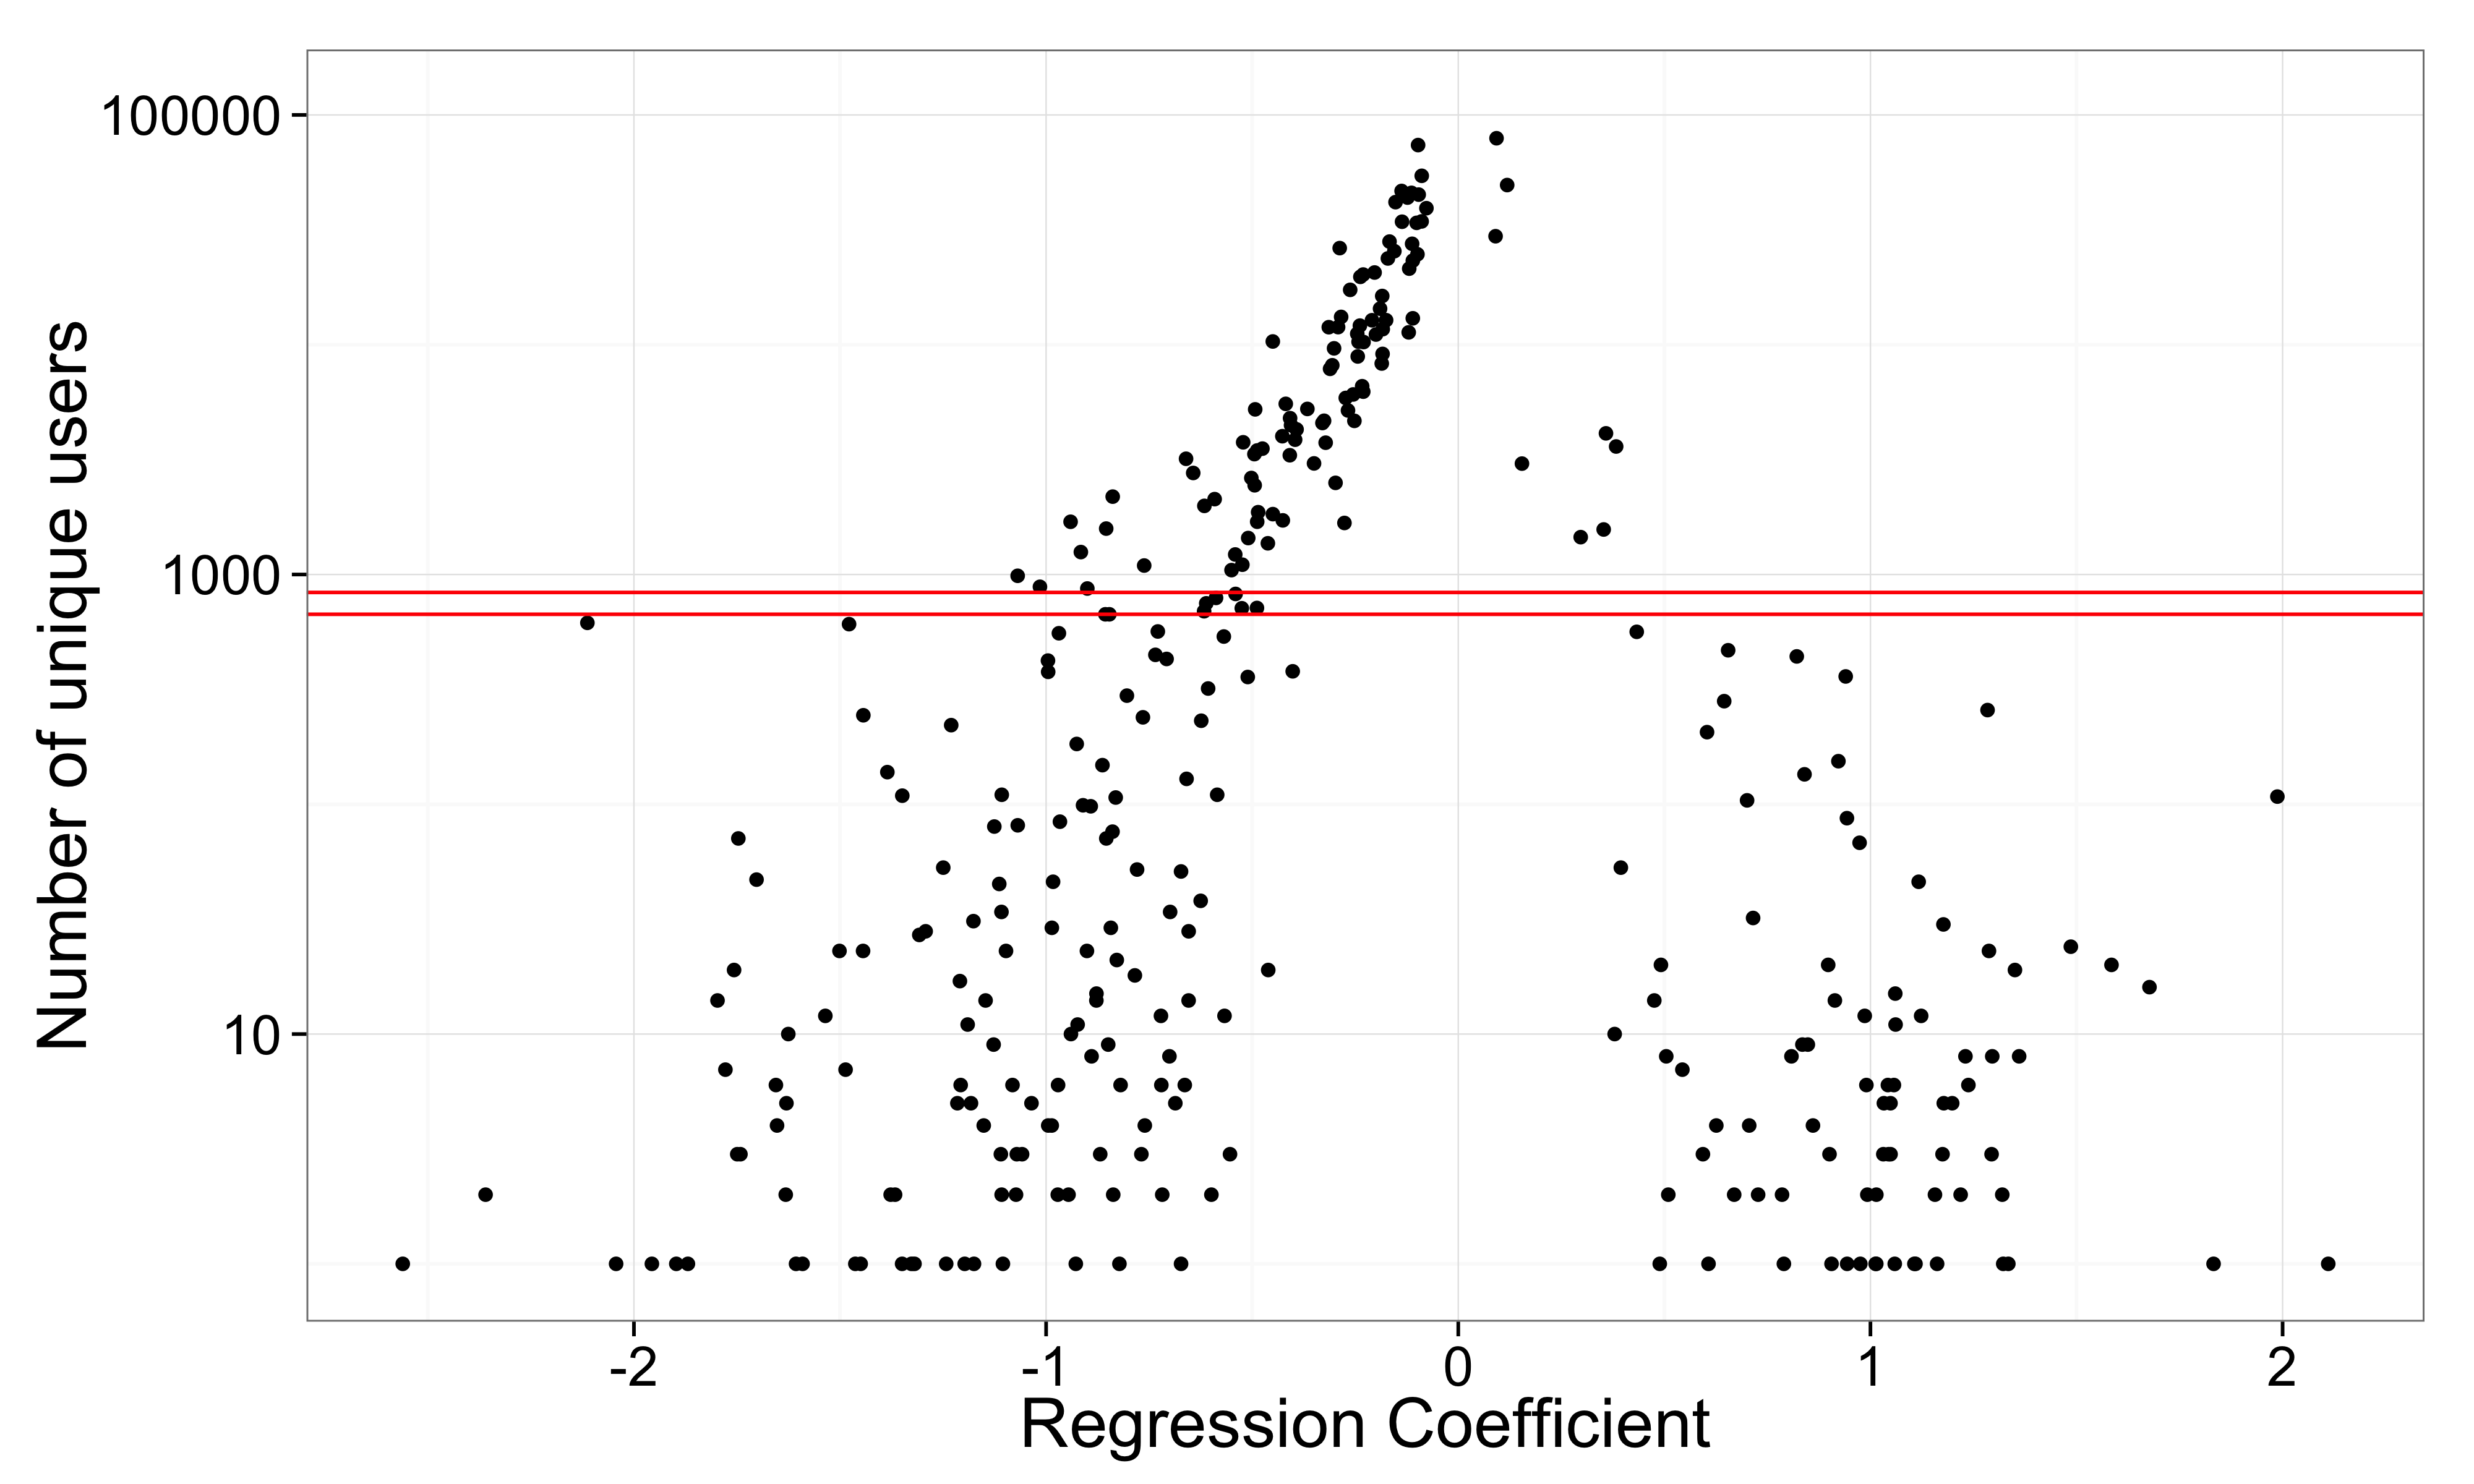
\includegraphics[width=0.45\textwidth]{tagRegressionWithMoreDataPeople.png}
    }
    \caption{In (a), the logarithm of tags' global popularity as a function of regression coefficient; in (b) the logarithm of number of unique users as a function of regression coefficient}
    \label{fig:secondPlotSet}
    \vspace{-1em}
  \end{figure}

The data suggest that the most popular tags under both metrics considered are significant, weakly positive predictors of future listening, while relatively unpopular tags tend to have relatively strong positive (and, in some cases, strong negative) impacts on listening. Tags which were not significant in the model had moderate to high popularity levels with respect to both the number of tags and the number of unique users who applied them. The high statistical reliability but small correlation coefficients for the most popular tags may be somwhat artifactual, primarily reflecting high variability in how predictive these these tags are of listening. We believe this finding is still informative, however, as it indicates that popular tags are not consistently associated with future listening.
%These data suggest that, at least for the small number of tags about which we can make statistically meaningful claims, those that are globally popular and well-known have relatively little effect on future listening, and are generally associated with small \emph{decreases} in post-taggging listening rates. The tags that seem to ``matter'' (i.e. those that are relatively strong predictors of whether or not a user will listen to an artist after tagging it) are generally much less popular.
\section{Conclusion}
\label{sec_conclusion}
In this paper we set out to test the oft-cited assumption that tags serve as retrieval aids for indivduals in collaborative tagging systems.  We did so via a novel methodology, testing for evidence that tagging an artist increases a user's future listening to that artist in comparison to a carefully selected set of untagged time series. Results suggest that tagging an artist does lead to an increase in listening, but that this increase is, on average, quite small (amounting to only 1 or 2 listens over a 6 month period). Given the various possible motivations for tagging, however, we expect only some tags to serve as retrieval cues, and thus tested the relative predictiveness of future listening for different tags. This analysis revealed systematic differences in how predictive the presence or absence of different tags was for future listening as a function of tag popularity. Specifically, we found that the most popular tags tend to have a small or non-significant effect on future listening, while less popular tags appear to be those that ``matter'', both as positive and negative predictors of future listening.

Based on such a small sample, we are at this point tentative to make strong claims about what specifically differntiates those unpopular tags that are strong negative versus strong positive predictors. The evidence is, nevertheless, suggestive of relatively uncommon (and likely, in many cases, to be idiosyncratic) tags being those most predictive of future listening behavior. This raises the intriguing possibility that the descriptive, popular tags that are arguably most useful to the community at large (i.e. genre labels and related tags), are not particularly associated with increases in listening, and thus are likely not functioning as memory cues.

This suggests that, while on average tagging an artist  has a small positive effect on future listening, the most common tagging activities are \emph{not} strong predictors of future retrieval. We cannot be sure which of the many other possible tagging motivations are at play here, nor can we know if and when a tag is applied with the intention of being used for retrieval, while ultimately not being used for this purpose. That said, these results do suggest that descriptive, relatively well-known genre classifiers do not show evidence of use as retrieval aids, but are nonetheless the most commonly applied tags. This may indicate that the primary motivation for tagging on Last.fm is not for personal information management (tagging a resource for one's own retrieval), but rather is socially-oriented, resulting in tags that are useful for the community at larger. This leads to the interesting possibility that a folksonomy can generate the useful, crowdsourced classification of content that proponents of collaborative tagging extol, but that this process is not strongly driven by the self-directed, retrieval-oritented tagging that is typically assumed in such systems.

While our results provide clues as to whether tags really function as retrieval aids, this remains early stage work addressing a hitherto unstudied research question. There is certainly room to refine and build upon the methods we present here for testing if and when tagging increases listening rates. In particular, our analysis at the level of artists (rather than the individual resources tagged) may be problematic, and we hope to eventually develop models that operate directly at the level of the content tagged (though data sparsity issues will make this a challenge). It will also be critical to expand on methods for understandings of which tags serve as memory cues and under what circumstances. It is clearly the case that not \emph{all} tags function as memory cues (and indeed, some curiously have an almost opposite effect), so more robustly identifying which tags do serve as memory retreival items is fruitful direction for future work. Incorporating research on human memory from the cognitive sciences can also further inform hypotheses and analytic approaches to these questions, something we are actively pursuing in ongoing research. A final limitation is that we are exploring tagging in a particular collaborative tagging system, which operates in the possibly idiosyncratic domain of music. Tagging habits may vary systematically in different cotent domains, but until usable data becomes avaialble, we can only speculate as to exactly how.

In closing, to address the titular question of whether or not tags function as retrieval aids, the best answer would appear to be ``sometimes''. While there is much work to be done on when and why particular tags serve this function and others do not, it is clear that the overarching retrieval assumption is far from valid: Tags certainly do not always function as memory cues, and our results suggest that retrieval may actually be among one of the least common of tagging motivations. 



\bibliographystyle{splncs}
\bibliography{references}

\end{document}
